\subsection{Плоскость}

\begin{wrapfigure}{r}{0.35\tw}
    \centering
    \vspace{-1pc}
    \tikzsetnextfilename{math-plane}
    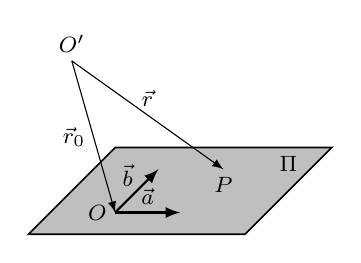
\begin{tikzpicture}[scale=1.1]
        \footnotesize

        \draw[semithick, fill=lightgray] (1, -1) -- (3.5, -1) -- (2.5, -2) -- (0, -2) -- cycle;

        \coordinate (O) at (0.5, 0);
        \coordinate (A) at (1, -1.75);
        \coordinate (B) at (2.25, -1.25);
        \coordinate (C) at (1.75, -1.75);
        \coordinate (D) at (1.5, -1.25);


        \draw[-latex] (O) -- (A);
        \draw[-latex] (O) -- (B);

        \draw[thick, -latex] (A) -- (C);
        \draw[thick, -latex] (A) -- (D);

        \point (O);
        \point (A);
        \point (B);

        \draw (O) node[anchor=south]{$O'$};
        \draw (A) node[anchor=east]{$O$};
        \draw (B) node[anchor=north]{$P$};

        \draw (1.375, -0.625) node[anchor=south]{$\vec{r}$};
        \draw (0.75, -0.875) node[anchor=east]{$\vec{r}_0$};
        \draw (1.375, -1.75) node[anchor=south]{$\vec{a}$};
        \draw (1.3, -1.55) node[anchor=south east]{$\vec{b}$};
        \draw (3.2, -1) node[anchor=north east]{$\Pi$};

    \end{tikzpicture}
    \caption{}
    \label{pic:math-plane}
\end{wrapfigure}
Аналогично предыдущему разделу, рассмотрим условие принадлежности точки $P$ с радиус-вектором $\vec{r}$ плоскости $\Pi$ в $\R^3$. Пусть неколлинеарные ($ \cross{a}{b} \not = 0$) векторы  $\vec{a}$ и $\vec{b}$~--- направляющие векторы плоскости $\Pi$, а точка $O$ с радиус-вектором $\vec r_0$ такова, что $\vec{r}_0 \in \Pi$. Тогда
\begin{equation}
    \vec{r} = \vec{r}_0 + \lambda\vec{a} + \mu\vec{b} \quad \Rightarrow \quad \begin{cases}
    x - x_0 = \lambda x_a + \mu x_b,\\
    y - y_0 = \lambda y_a + \mu y_b,\\
    z - z_0 = \lambda z_a + \mu z_b;
\end{cases}\quad \lambda, \mu \in \R.
\end{equation}
Преобразуем полученную систему уравнений:
\begin{align*}
& \left\{
\begin{aligned}
    \lambda &= \dfrac{x - x_0 - \mu x_b}{x_a},\\
    y - y_0 &= \dfrac{x - x_0 - \mu x_b}{x_a} \cdot y_a + \mu y_b,\\
    z - z_0 &= \lambda z_a + \mu z_b.
\end{aligned}\right.\\
& \left\{
\begin{aligned}
    \lambda &= \dfrac{x - x_0 - \mu x_b}{x_a},\\
    y - y_0 &= (x - x_0) \cdot \dfrac{y_a}{x_a} + \mu \left(y_b - \dfrac{x_b y_a}{x_a} \right),\\
    z - z_0 &= \lambda z_a + \mu z_b.
\end{aligned}\right.\\
&\left\{
\begin{aligned}
    \lambda &= \dfrac{x - x_0 - \mu x_b}{x_a},\\
    \mu &= \dfrac{x_a y - x_a y_0 - (x - x_0) \cdot y_a}{x_a y_b - x_b y_a},\\
    z - z_0 &= \lambda z_a + \mu z_b.
\end{aligned}\right.
\end{align*}
Подставим выражения для $\lambda$ и $\mu$ в третье уравнение:
\begin{multline*}
    z - z_0 = \dfrac{x - x_0 - \mu x_b}{x_a} \cdot z_a + \mu z_b = (x - x_0) \cdot \dfrac{z_a}{x_a} + \mu \left( z_b - \dfrac{x_b z_a}{x_a} \right) = \\
    = (x - x_0) \cdot \dfrac{z_a}{x_a} + \dfrac{x_a y - x_a y_0 - (x - x_0) \cdot y_a}{x_a y_b - x_b y_a} \cdot \left( z_b - \dfrac{x_b z_a}{x_a} \right)
\end{multline*}
Приведя подобные слагаемые с $x$, $y$ и $z$, получим:
\begin{multline*}
z = x \cdot \underbrace{\left( \dfrac{z_a}{x_a} - \dfrac{y_a}{x_a y_b - x_b y_a} \left( z_b - \dfrac{x_b z_a}{x_a} \right) \right)}_A +\\
+ y \cdot \underbrace{\dfrac{x_a}{x_a y_b - x_b y_a} \cdot \left( z_b - \dfrac{x_b z_a}{x_a} \right)}_B +\\
+ \underbrace{z_0 - \dfrac{x_0 z_a}{x_a} - \dfrac{x_a y_0 - x_0 y_a}{x_a y_b - x_b y_a} \cdot \left( z_b - \dfrac{x_b z_a}{x_a} \right)}_D.
\end{multline*}
Сделаем замену:
\begin{align*}
&
\begin{aligned}
    A \equiv  \dfrac{z_a}{x_a} &- \dfrac{y_a}{x_a y_b - x_b y_a} \left( z_b - \dfrac{x_b z_a}{x_a} \right) = \\
    &\quad\quad= \frac{x_a y_b z_a - x_b y_a z_a}{x_a (x_a y_b - x_b y_a)} - \frac{x_a y_a z_b - x_b y_a z_a}{x_a (x_a y_b - x_b y_a)} = \frac{y_b z_a - y_a z_b}{x_a y_b - x_b y_a},
\end{aligned}\\
&
B \equiv \dfrac{x_a}{x_a y_b - x_b y_a} \cdot \left( z_b - \dfrac{x_b z_a}{x_a} \right) 
%= \frac{x_a (x_a z_b - x_b z_a)}{x_a (x_a y_b - x_b y_a)} = 
\frac{x_a z_b - x_b z_a}{x_a y_b - x_b y_a},\\
&
D \equiv z_0 - \dfrac{x_0 z_a}{x_a} - \dfrac{x_a y_0 - x_0 y_a}{x_a y_b - x_b y_a} \cdot \left( z_b - \dfrac{x_b z_a}{x_a} \right).
\end{align*}
В результате такой замены получим уравнение
\begin{equation}
Ax + By - z + D = 0.
\end{equation}
Домножим в нём обе части на $\xi \equiv x_a y_b - x_b y_a$ и сделаем ещё одну замену:
\begin{equation*}
A'x + B'y + C'z + D' = 0,
\end{equation*}
где $D' = \xi D$, а
\begin{equation*}
\begin{cases}
    A' = y_b z_a - y_a z_b = \det
    \begin{pmatrix}
        y_b & z_b\\
        y_a & z_a
    \end{pmatrix}\\[1pc]
    B' = x_a z_b - x_b z_a = \det
    \begin{pmatrix}
        x_a & z_a\\
        x_b & z_b
    \end{pmatrix}\\[1pc]
    C' = x_b y_a - x_a y_b = \det
    \begin{pmatrix}
        x_b & y_b\\
        x_a & y_a
    \end{pmatrix}
\end{cases}
\end{equation*}
Легко видеть, что
\begin{equation}
\begin{pmatrix}
    A'\\
    B'\\
    C'
\end{pmatrix} =
\cross{b}{a} \equiv \vec{n}.
\end{equation}
Из свойств векторного произведения вектор $\vec n$ является \imp{вектором нормали} к плоскости $\Pi$.

Теперь  самое первое условие можно записать так:
\begin{equation}
\scalar{r}{n} = \triple{r}{b}{a} = -D' = (\vec{r}_0, \vec{b}, \vec{a}).
\end{equation}
